\documentclass[a4paper,12pt]{article}

\usepackage[utf8]{inputenc}
\usepackage[french]{babel}
\usepackage{footnote}
\usepackage{hyperref}
\usepackage{graphicx}
\usepackage{tikz}
\usepackage{fancyhdr}
\usepackage[numbers]{natbib}
\usepackage{amssymb}
\usepackage{amsmath}
\usepackage[linesnumbered,ruled,vlined,noend,french,onelanguage]{algorithm2e}
\usepackage{listings}
\usepackage{xcolor}
\usepackage{adjustbox}
\usepackage{float}
\usepackage[T1]{fontenc}
\usepackage{natbib}
\usepackage{subcaption}

\SetKwComment{Comment}{// }{}
\SetKwProg{Fn}{Fonction}{ :}{}

\usetikzlibrary{positioning}
\usetikzlibrary{calc}
\usetikzlibrary{math}
\usetikzlibrary{arrows}

\pagestyle{fancy}

\textheight 26cm      
\textwidth 16.0cm      
\oddsidemargin 2.5cm            
\evensidemargin 2.5cm          
\addtolength{\oddsidemargin}{-2.5cm}
\addtolength{\evensidemargin}{-2.5cm}
\topmargin 0 cm      
\addtolength{\topmargin}{-2cm}  

\fancyhfoffset[L]{0.1in} % Ajuster la marge gauche de l'en-tête
\fancyhfoffset[R]{0.1in} % Ajuster la marge droite de l'en-tête

\renewcommand{\headrulewidth}{1pt}
\fancyhead[R]{Année universitaire: 2024-2025}
\fancyhead[L]{Pedro Henrique Rodriguez Russo - Jo\~ao Pedro Neto de Abreu}

\renewcommand{\footrulewidth}{1pt}
\fancyfoot[C]{\thepage} 
\fancyfoot[L]{ENSEIRB-MATMECA}
\fancyfoot[R]{TP Analyse du Cycle de Vie }

\newcommand\blankpage{%
    \null
    \thispagestyle{empty}%
    \addtocounter{page}{-1}%
    \newpage}



\title{Application K-Moyennes}

\author{NETO DE ABREU Jo\~ao Pedro \\ RODRIGUEZ RUSSO Pedro Henrique}
\date{}

\begin{document}

\maketitle

\begin{center}
  \large
  EISIS102 - Traitement de l'Information \\
  Département Informatique\\
  S5 - Année 2024/2025\\
  \vfill
  
\includegraphics[width=0.2\textwidth]{enseirb-matmeca.png}
\end{center}

\newpage

\tableofcontents

\newpage

\section{Introduction}
Ce rapport concerne le traitement de données publiques issues d'un site de base données pour appliquer au machine learning \footnote{\url{https://archive.ics.uci.edu/}}. Pour analyser ces données, qui sont de types ratio, nous avons choisi d'utiliser deux méthodes :\\
\begin{enumerate}
\item On appliquera d'abord un ACP afin de réduire le nombre de caractéristiques pour ensuite appliquer l'algorithme des K-moyennes pour trouver les 3 cépages differents.\\
\item On applique directement l'algorithme des K-moyennes.
\end{enumerate}
\vspace{1cm}
Dans la section \ref{sec:presentation1}, nous présentons la base de données utilisée.Nous décrivons alors la méthode d'analyse de données considérée en section \ref{sec:presentation2}. Puis, on analysera les résultats obtenues dans la section \ref{sec:analyse}. Une conclusion sur le travail réalisé est enfin proposée en section \ref{sec:conclusion}.

\section{Présentation des données}
\label{sec:presentation1}
Cette base de données résulte d'une étude chimique des vins produit dans la même région italienne. Cette base de données rassemble des données concernant des vins issus de trois variétés distinctes. Les informations ont été collectées afin d'analyser la composition chimique et de fournir un cadre pour des analyses statistiques, en particulier en apprentissage automatique. Les informations sont issues de l'étude de 13 composés chimiques présents dans chaque type de vin.

%\newpage

\section{Présentation de la méthode}
\label{sec:presentation2}
\subsection{Analyse en Composantes Principales (ACP)}

La méthode d'analyse statistique appelée Analyse en Composantes Principales (ACP) vise à diminuer la dimensionnalité d'un jeu de données tout en préservant un maximum d'informations. Grâce à elle, il est possible de convertir des variables corrélées en un ensemble de variables non corrélées appelées composantes principales.\\

\subsubsection{Objectif}

L'ACP vise à diminuer la quantité de caractéristiques (ou de dimensions) tout en préservant l'information la plus pertinente. L'amélioration des performances des algorithmes de traitement est facilitée par cette réduction. \\

\subsubsection{Principe fonctionnement}

On a une matrice X $ \in \mathbb{R}^{n\times p}$ qui contient les données quantitative. On note x$_i$ la i$^{\text{ième}}$ ligne et x$^j$ la j$^{\text{ième}}$ colonne.\\

\begin{equation}
  \text{On calcule, } \forall j \in \llbracket 0, p \rrbracket, \quad \mu_j = \frac{1}{n} \sum_{i=1}^nx_i^j
\end{equation}
\begin{equation}
  \text{Puis, } \forall j \in \llbracket 0, p \rrbracket, \quad \sigma_j^2 = \frac{1}{n} \sum_{i =1}^n (s_i^j - \mu_j )^2
\end{equation}
\begin{equation}
  \text{Enfin, on standardise les données : } \forall (i, j) \in \llbracket 0, n \rrbracket \times \llbracket 0, p \rrbracket, \quad \tilde{x}_i^j = \frac{ x_i^j - \mu^j}{\sigma_j}
\end{equation}
\vspace{10pt}
Après avoir standardiser les données \~X, on calcule la matrice de correlation:
\begin{equation}
  C = \frac{1}{n}\tilde{X}^T\tilde{X}
\end{equation}

Après avoir calculé C, on trouve les valeurs propres et les vecteurs propres associés pour ensuite regarder les valeurs propres et garder celles qu'on souhaite avec les deux méthodes possibles : soit la méthode du coude, c'est-à-dire une grande diminution d'une valeur propre à la suivante, soit en gardant 95 \% de la variance.


\subsection{K-Moyennes}
L'algorithme de classification non supervisée K-moyenne est une technique de clustering qui permet de regrouper des données en un nombre prédéfini de groupes (clusters).

\subsubsection{Objectif}
Composer des groupes homogènes d'observations similaires.\\

Chaque point est attribué au cluster le plus proche dont le centre (centroïde).

\subsubsection{Principe de fonctionnement}

\begin{algorithm}[h!]
  \small
  \caption{Pseudo-code de K-Moyenne}
  K\_MOYENNES(Z,k):\\
  \KwData{Z = ensemble de points, k = un entier}
  \KwResult{Une liste contenant les k cluster avec leur point}
  B = Tableau de k listes  \\
  B' = Copie de B\\
  m$_1$, $\cdots$, m$_k$ = Tirage au hasard dans Z\\
  \ForAll{x $\in$ Z}{
    j$_{min}$ = j tel que dist(x,m$_j$) est minimale \\
    Ajout de x à B[j$_{min}$] \\
  }
  \While{ B $\neq$ B'}{
    B' = copie de B\\
    \For{j=1 to k:}{
      m$_j$ = moyenne des éléments de B[j]
    }
    B = Tableau de k listes vides\\
    \ForAll{x $\in$ Z}{
      j$_{min}$ = j tel que dist(x,m$_j$) est minimale \\
      Ajout de x à B[j$_{min}$] \\
    }
  }
  \Return B
\end{algorithm}

\newpage

\section{Analyse des résultats obtenues}
\label{sec:analyse}

\subsection{Analyse de Composantes Principales + K-Moyennes}

Lorsqu'on trie le tableau contenant les valeurs propres de la matrice de correlation, on obtient le graphe suivant: \\

\begin{figure}[h!] % Placement de l'image
   \centering
   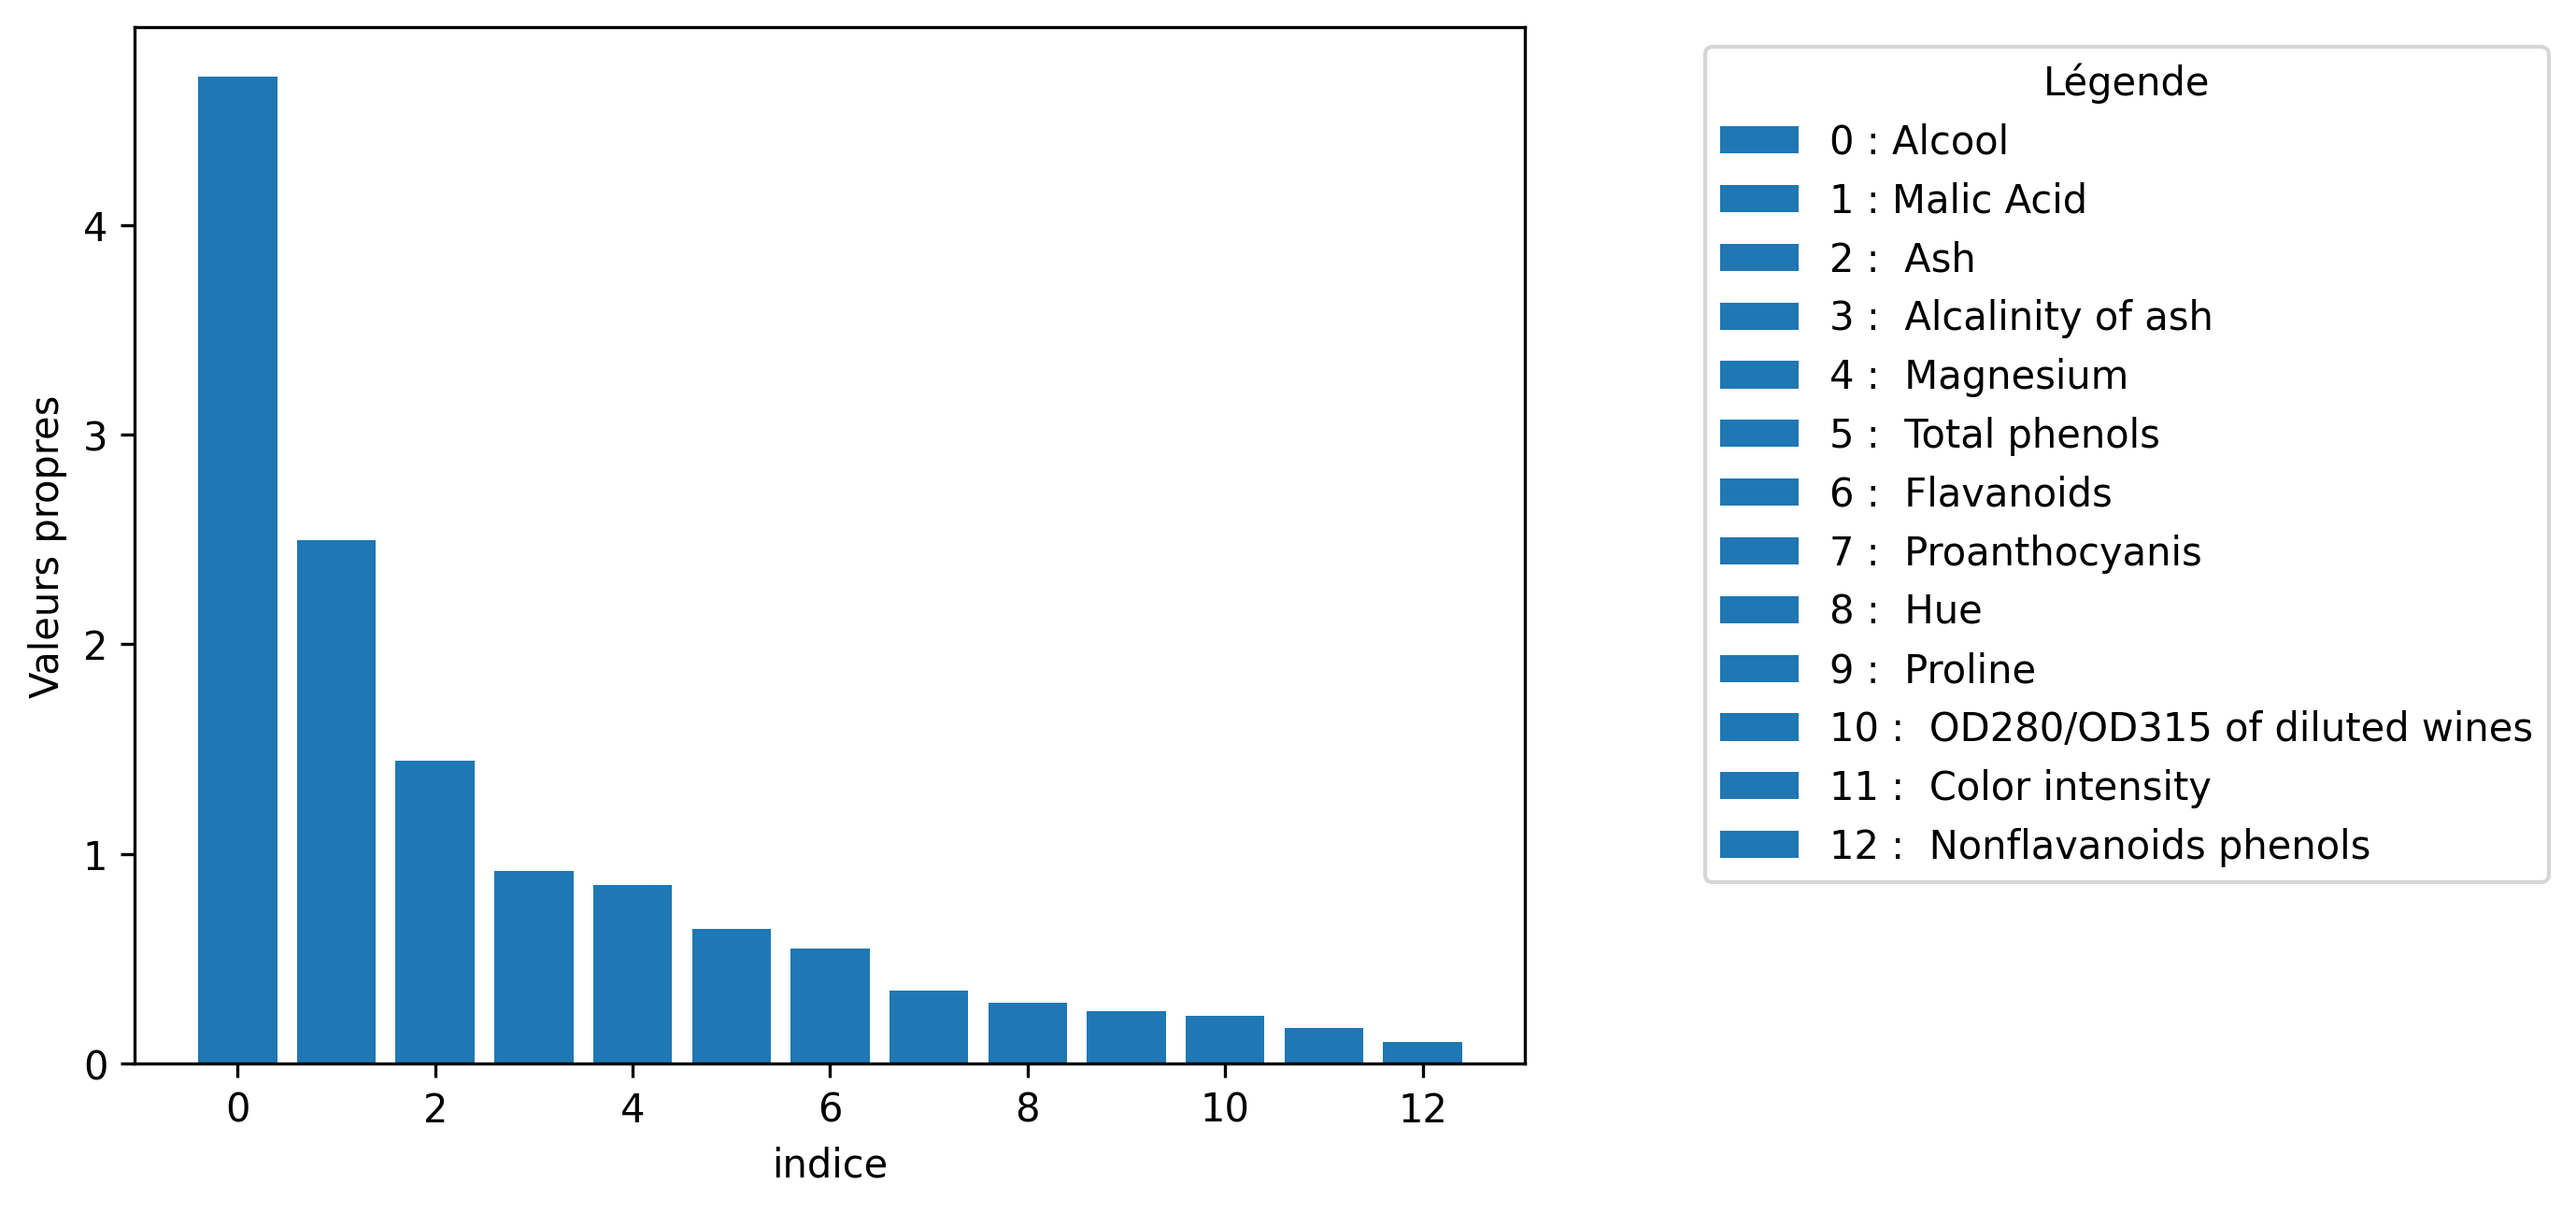
\includegraphics[width=0.8\textwidth]{vp.png} % Chemin de l'image
   \caption{Valeurs propres trièes dans l'ordre décroissante}
   \label{fig:vp} % Label pour faire référence à l'image
\end{figure}  
             
Comme on n'a pas de grande diminution d'une valeur propre à la suivante, on va donc prendre l'autre méthode pour savoir le nombre caractéristiques à garder. Après calcul on obtient 8 caractéristiques au lieu de 13.\\

Dans le module KMeans, il y a deux algorithmes disponibles pour calculer les cluster de nos données.

\begin{figure}[h!] % Placement de l'image
  \centering
  \begin{subfigure}[b]{0.48\textwidth}
    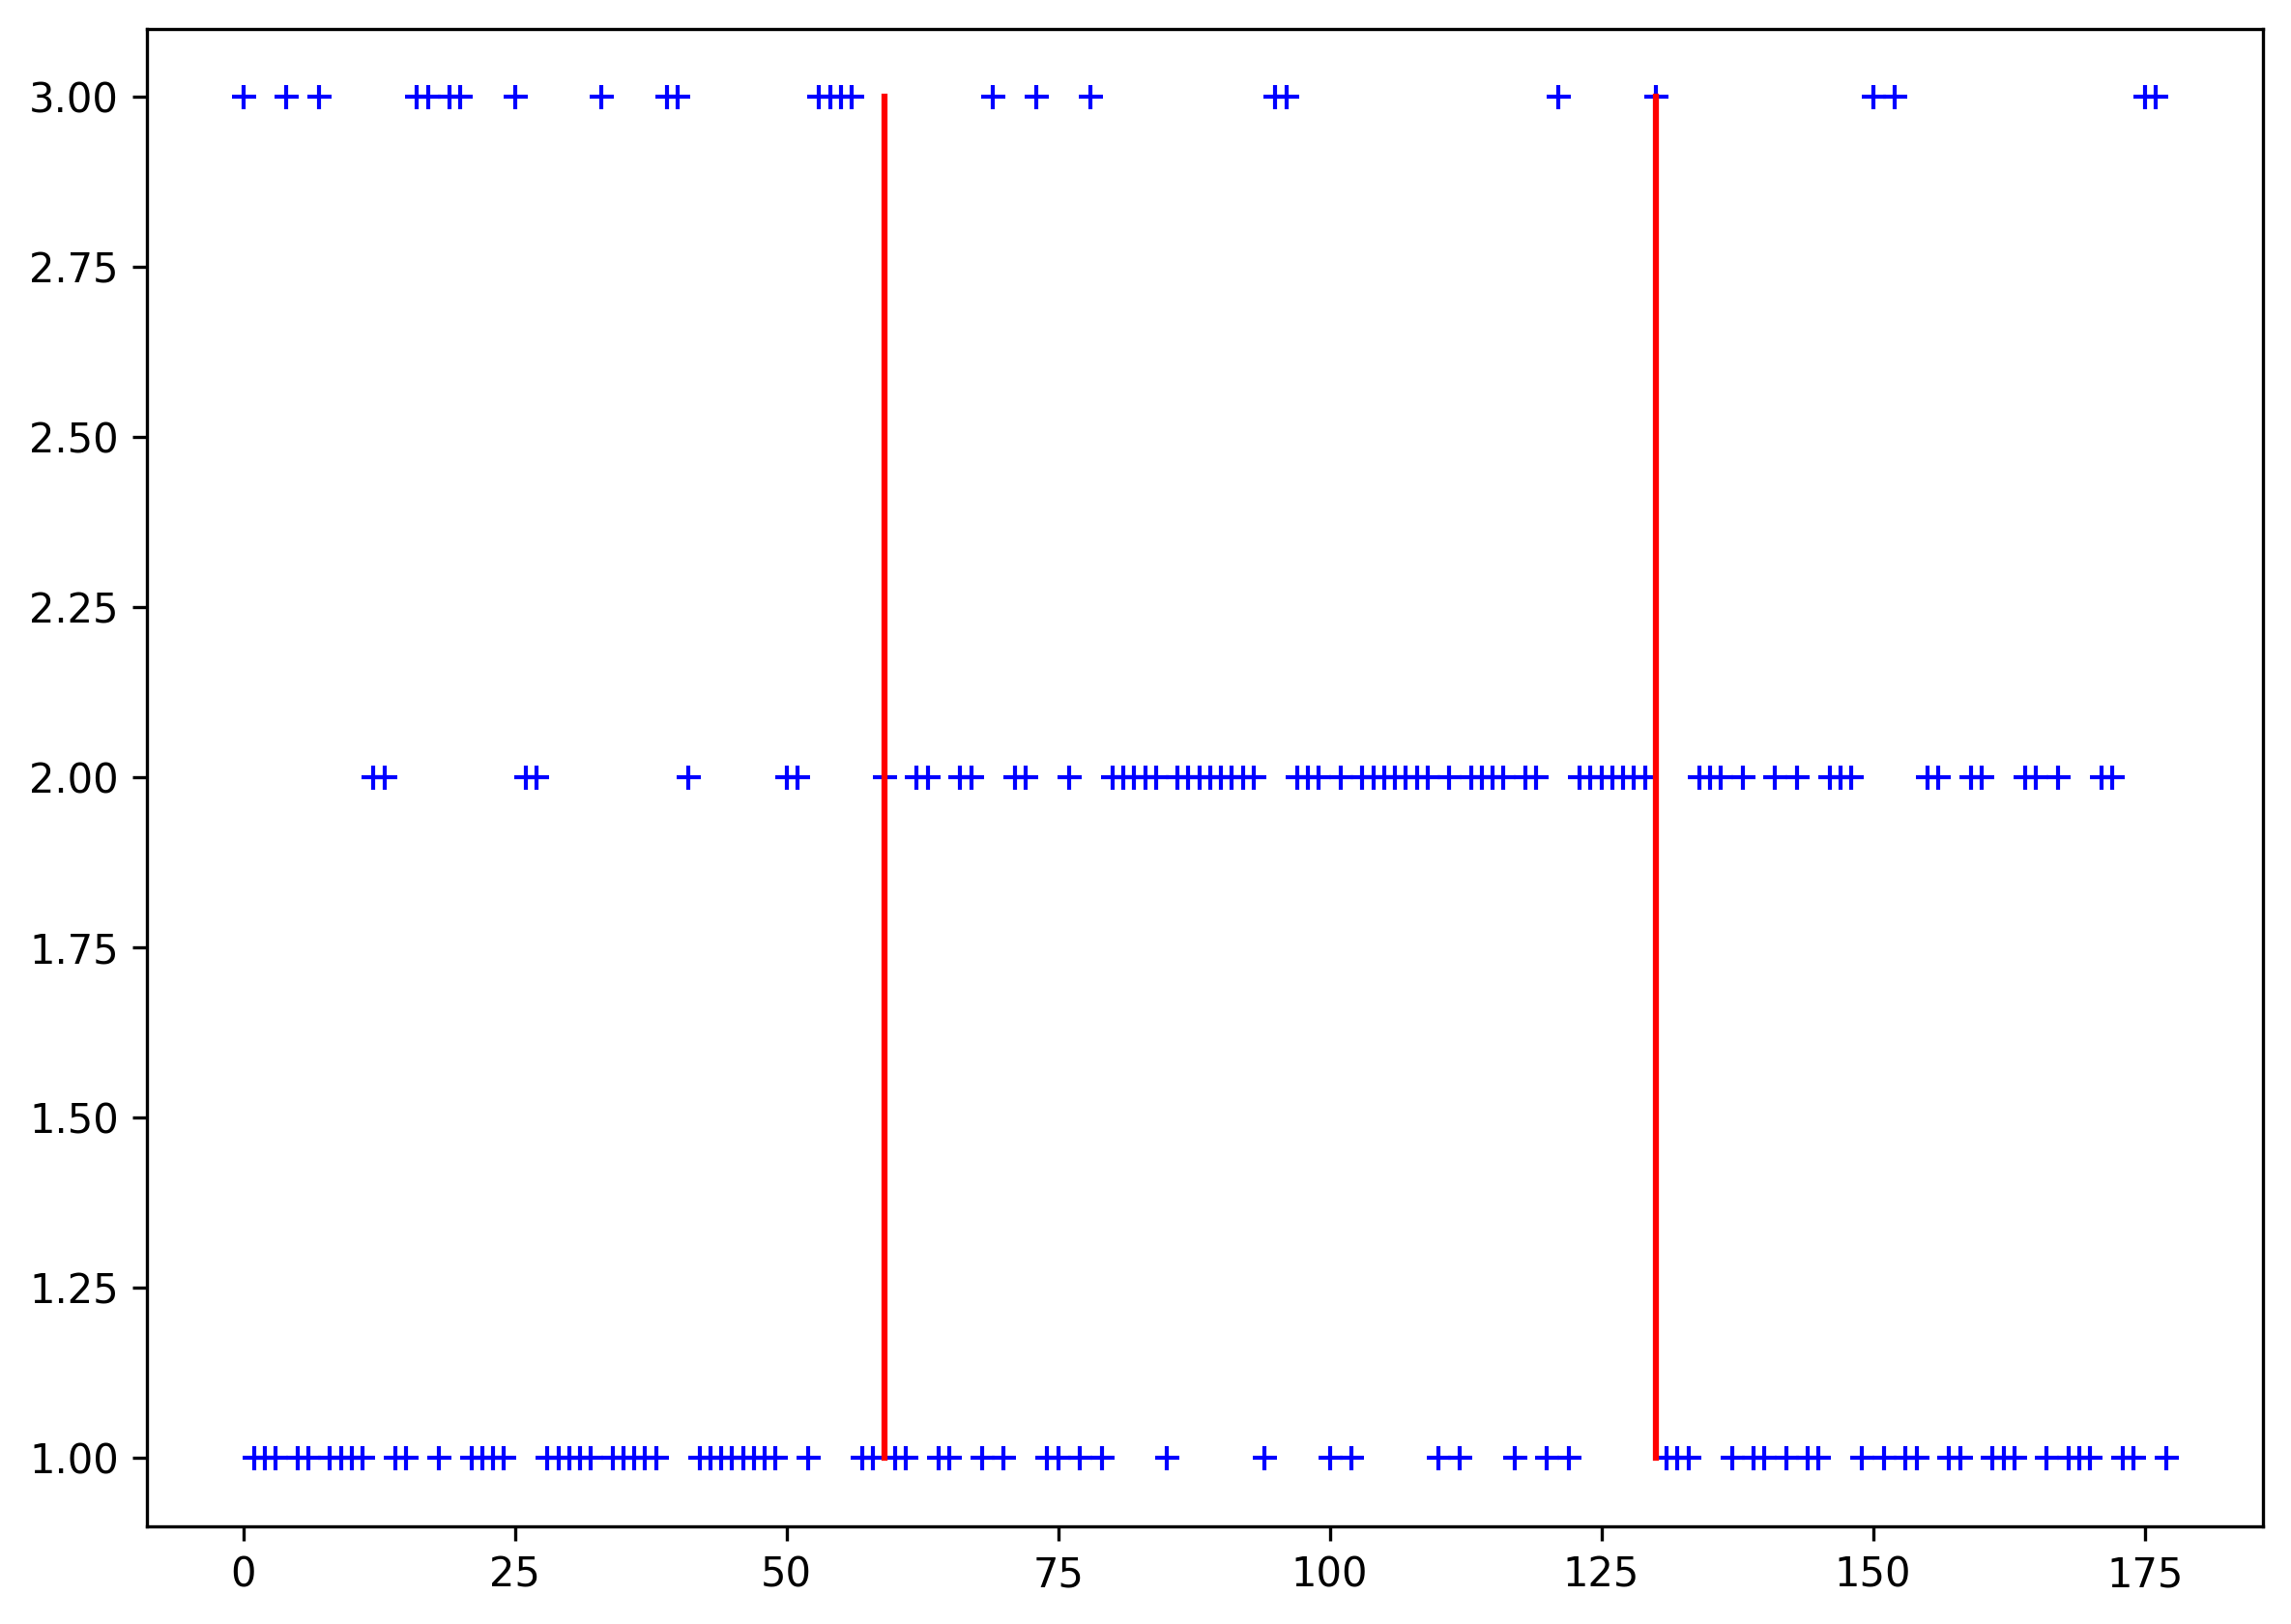
\includegraphics[width=\textwidth]{lloyd.png} % Chemin de l'image
    \caption{Classes des données avec l'algorithme de Lloyd}
    \label{fig:lloyd} % Label pour faire référence à l'image
  \end{subfigure}
  \hfill
  \begin{subfigure}[b]{0.48\textwidth}
    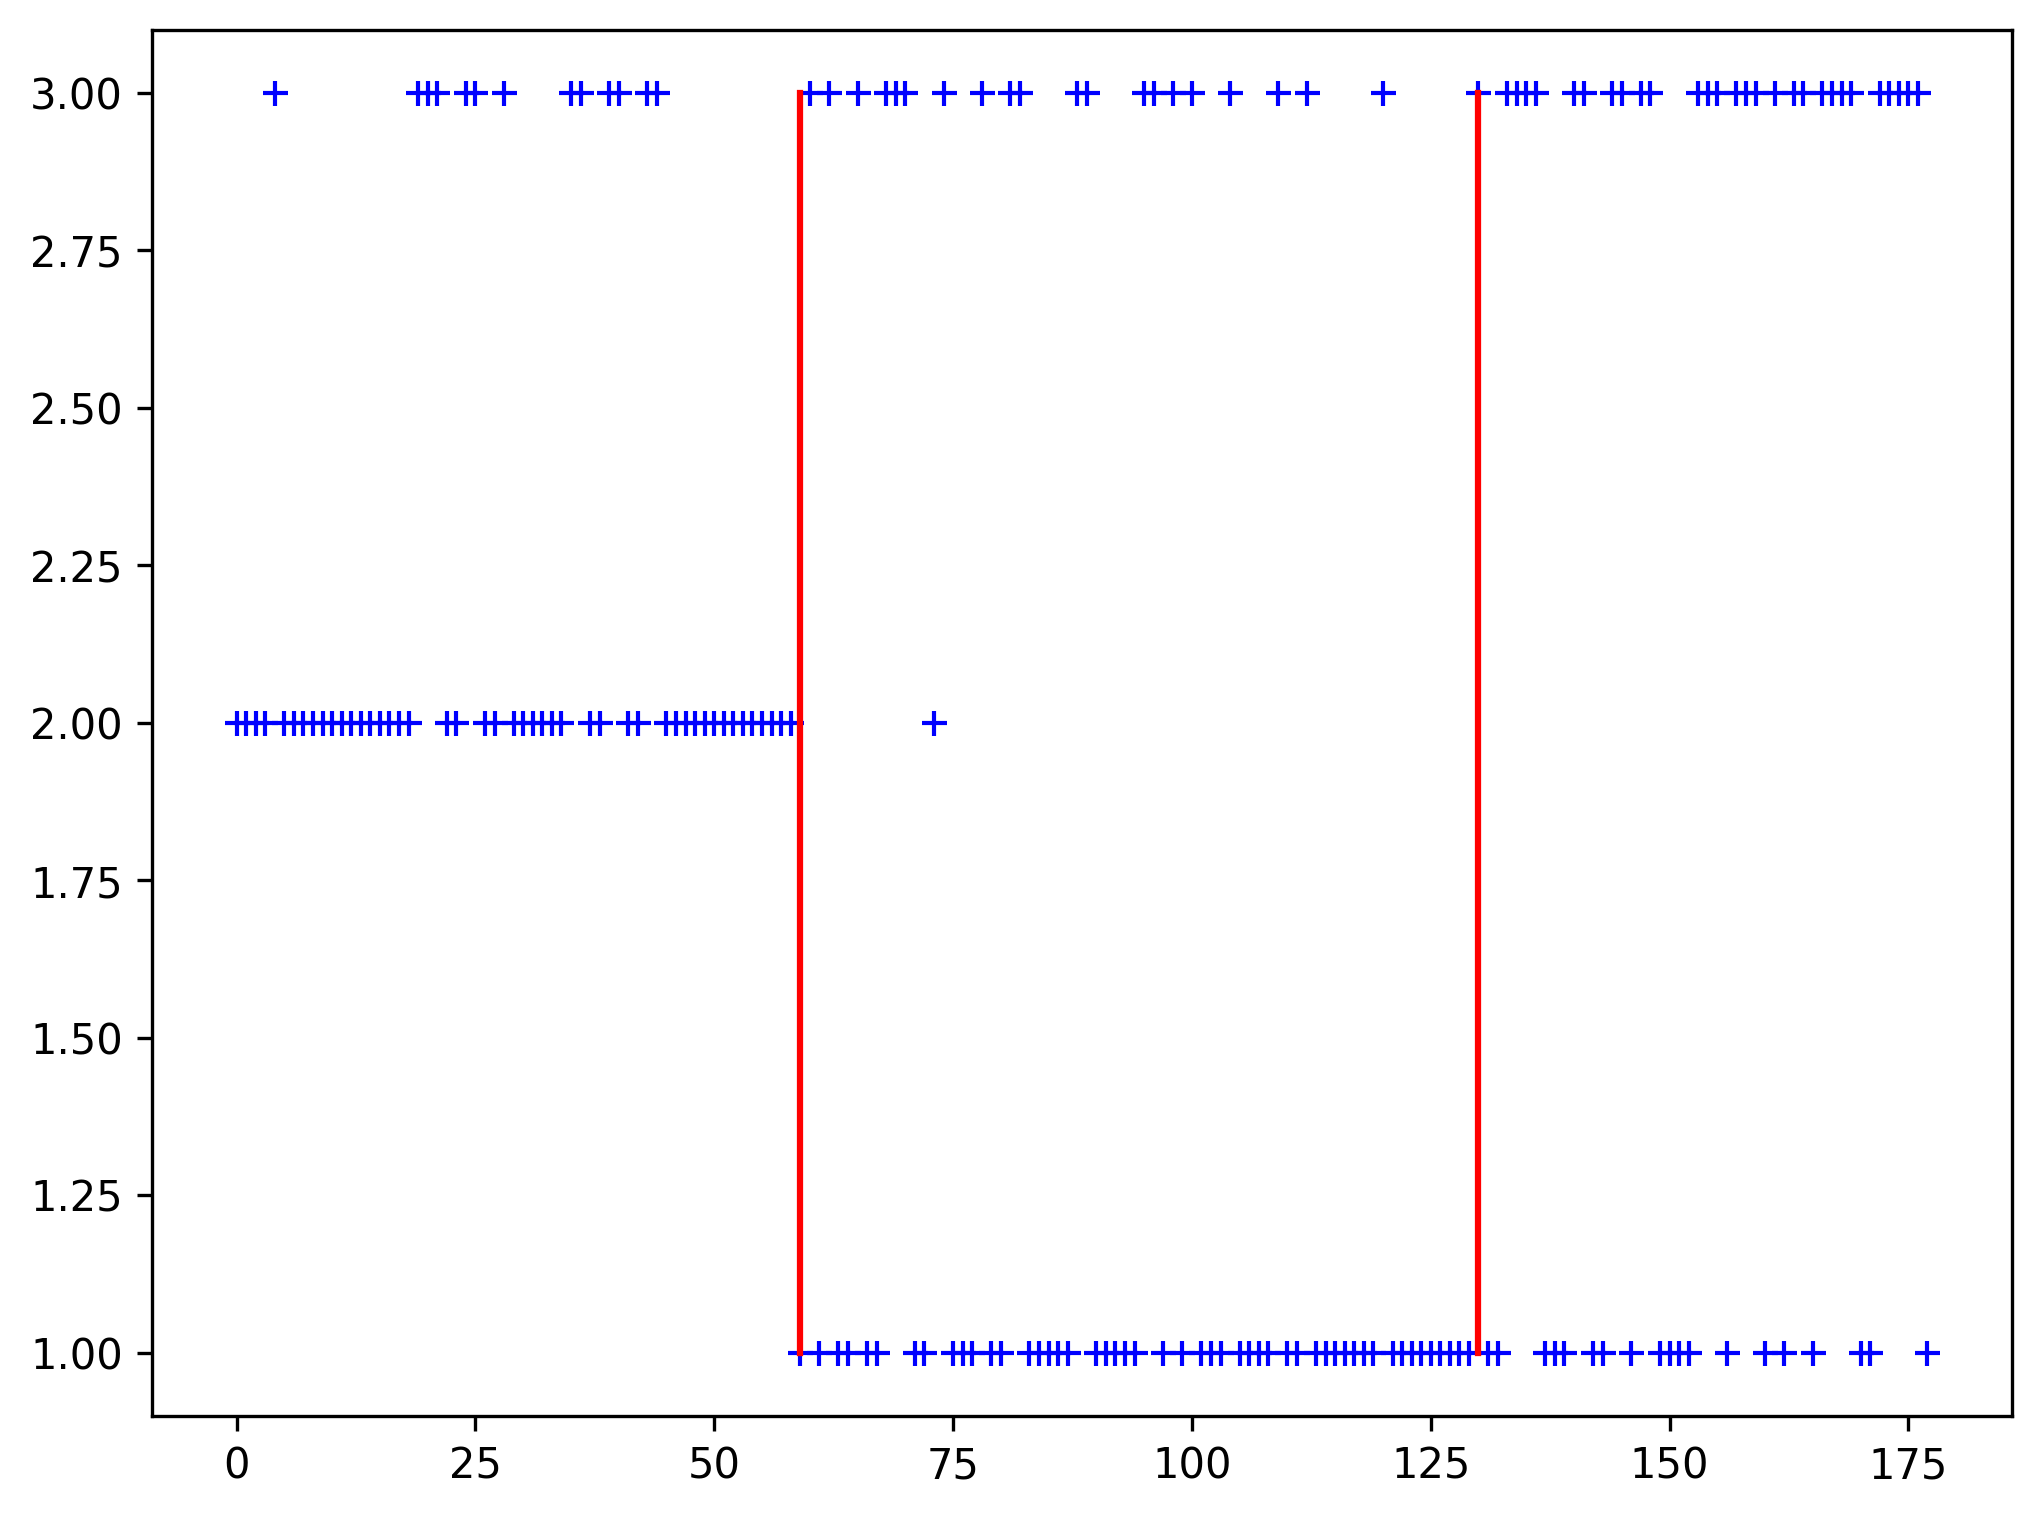
\includegraphics[width=\textwidth]{elkan.png} % Chemin de l'image
    \caption{Classes des données avec l'algorithme d'Elkan}
    \label{fig:elkan} % Label pour faire référence à l'image
  \end{subfigure}
  \label{fig:deux_images}
\end{figure}

Voici les taux de succès de chaque algorithme: \\
\begin{table}[h!]
  \centering
  \begin{tabular}{| c | c | c |}
    \hline & Lloyd & Elkan \\ \hline
    Total & 49.44 \% & 49.44 \% \\ \hline
    Classe 1 & 62.71 \% & 62.71 \% \\ \hline
    Classe 2 & 64.79 \% & 64.79 \% \\ \hline
    Classe 3 & 10.42 \% & 10.42 \% \\ \hline
  \end{tabular}
\end{table}

\subsection{K-Moyennes seule}
\subsubsection{Utilisation de toutes les données}
En utilisant toutes les données fournies par le tableau on applique dirrectement les K-Moyennes avec les algorithmes Elkan et Lloyd.
\newpage

\begin{figure}[h!] % Placement de l'image
   \centering
   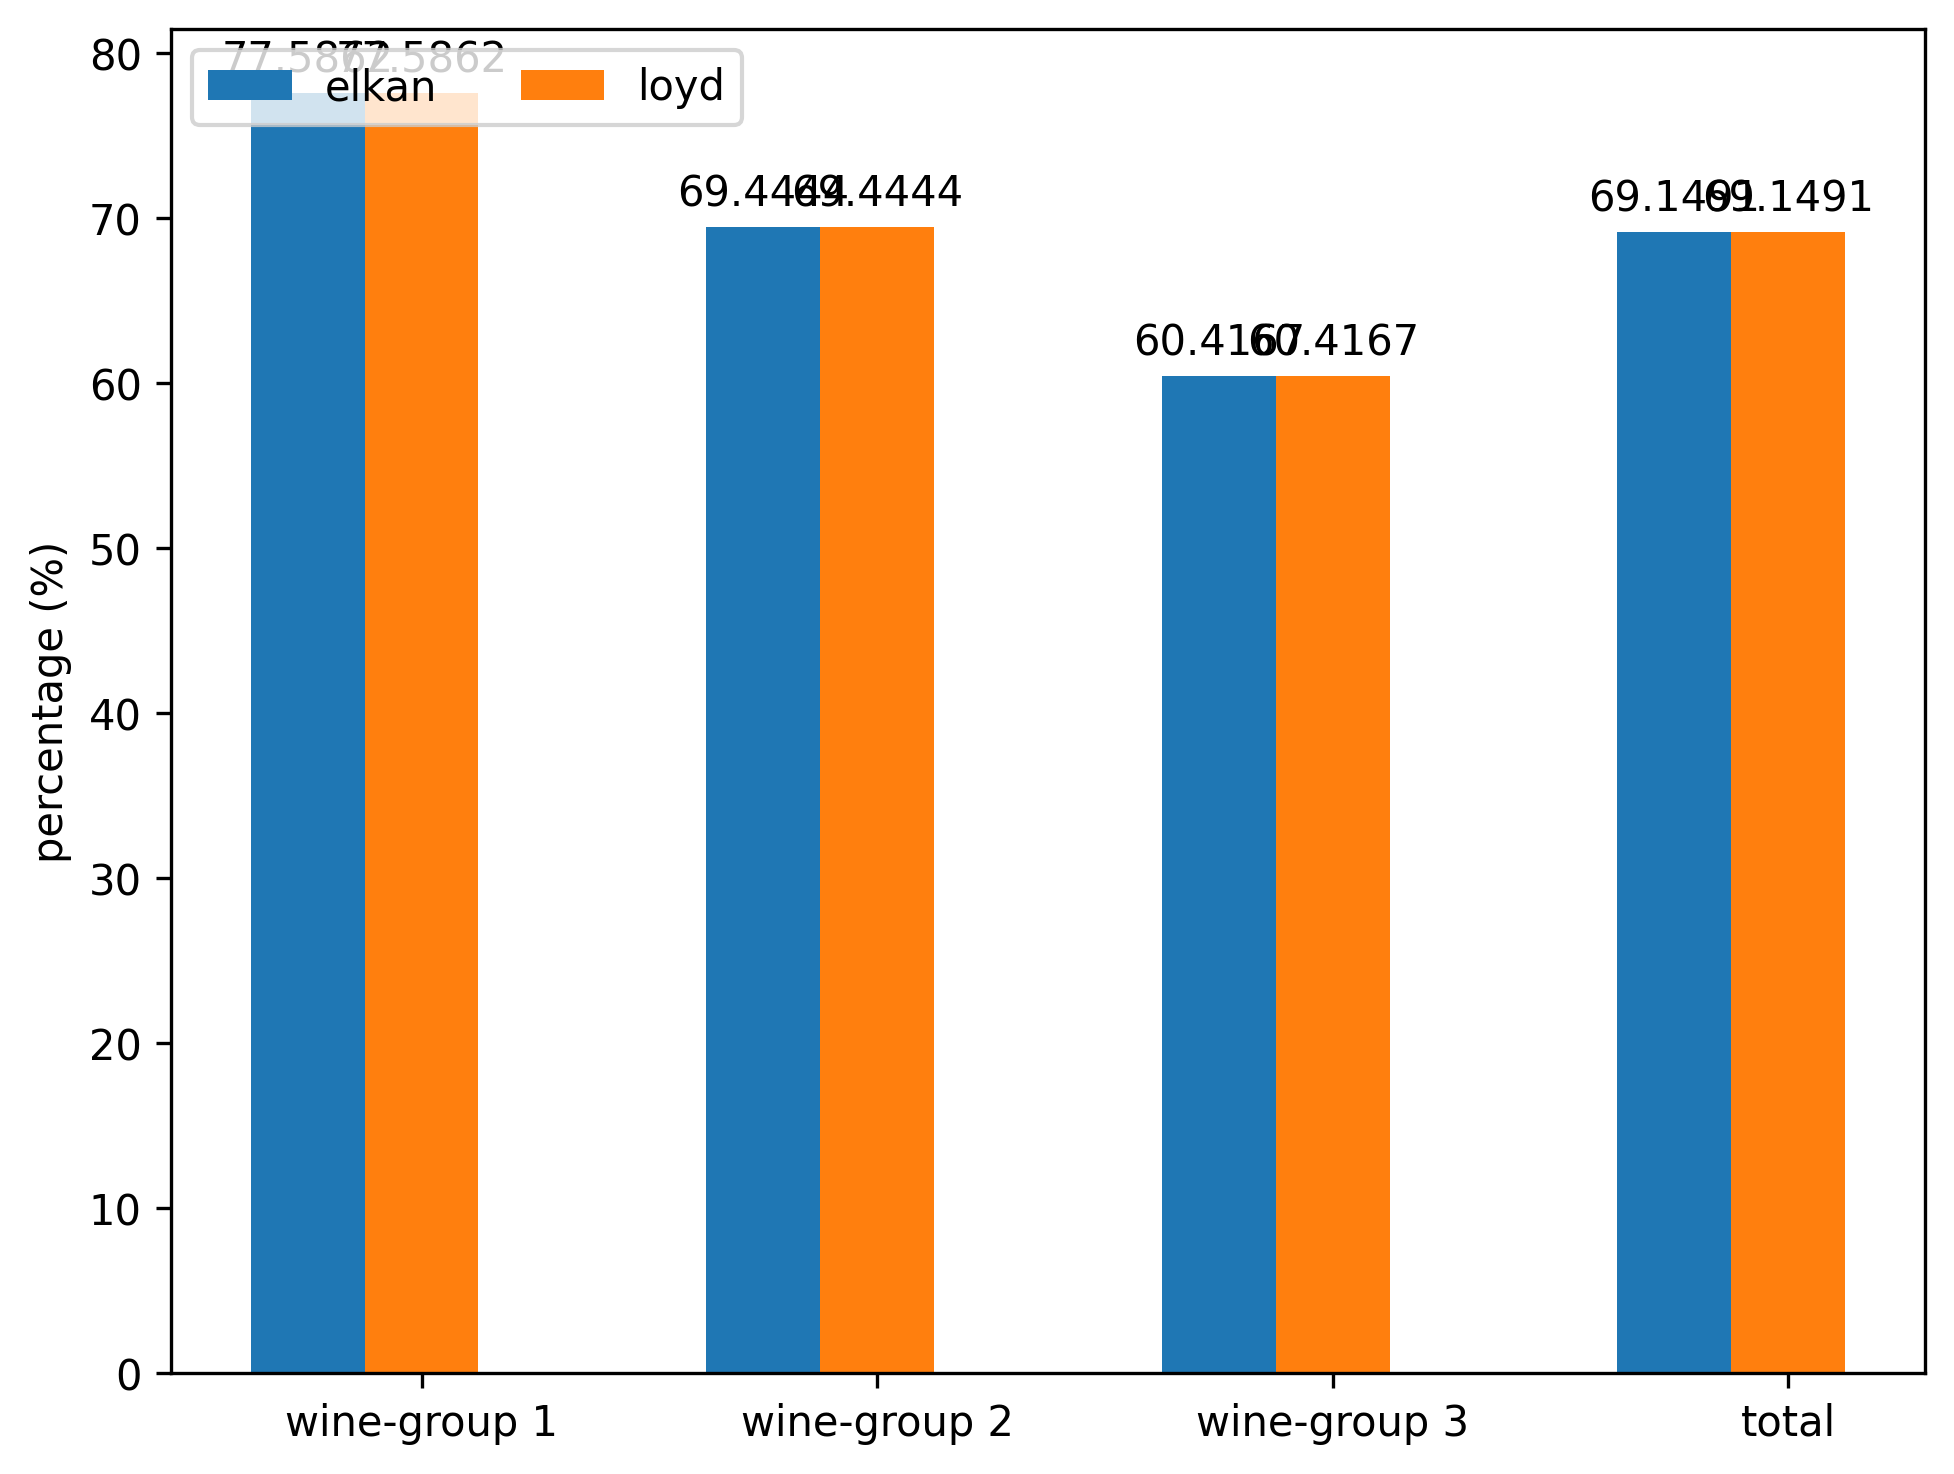
\includegraphics[width=0.6\textwidth]{comparaison_algos.png} % Chemin de l'image
   \caption{Resultats obtenues par les algorithmes lloyd et elkan}
   \label{comparaison_algos.png} % Label pour faire référence à l'image
\end{figure}

On remarque que les deux algorithmes donnent le même résultat. Pour la suite du projet on utilisera donc l'algorithme de lloyd.

\subsubsection{Utilisation donnes specifiques}

Lorsqu'on applique KMeans avec des attributs choisis par une personne lambda on obtient :

\begin{figure}[h!] % Placement de l'image
   \centering
   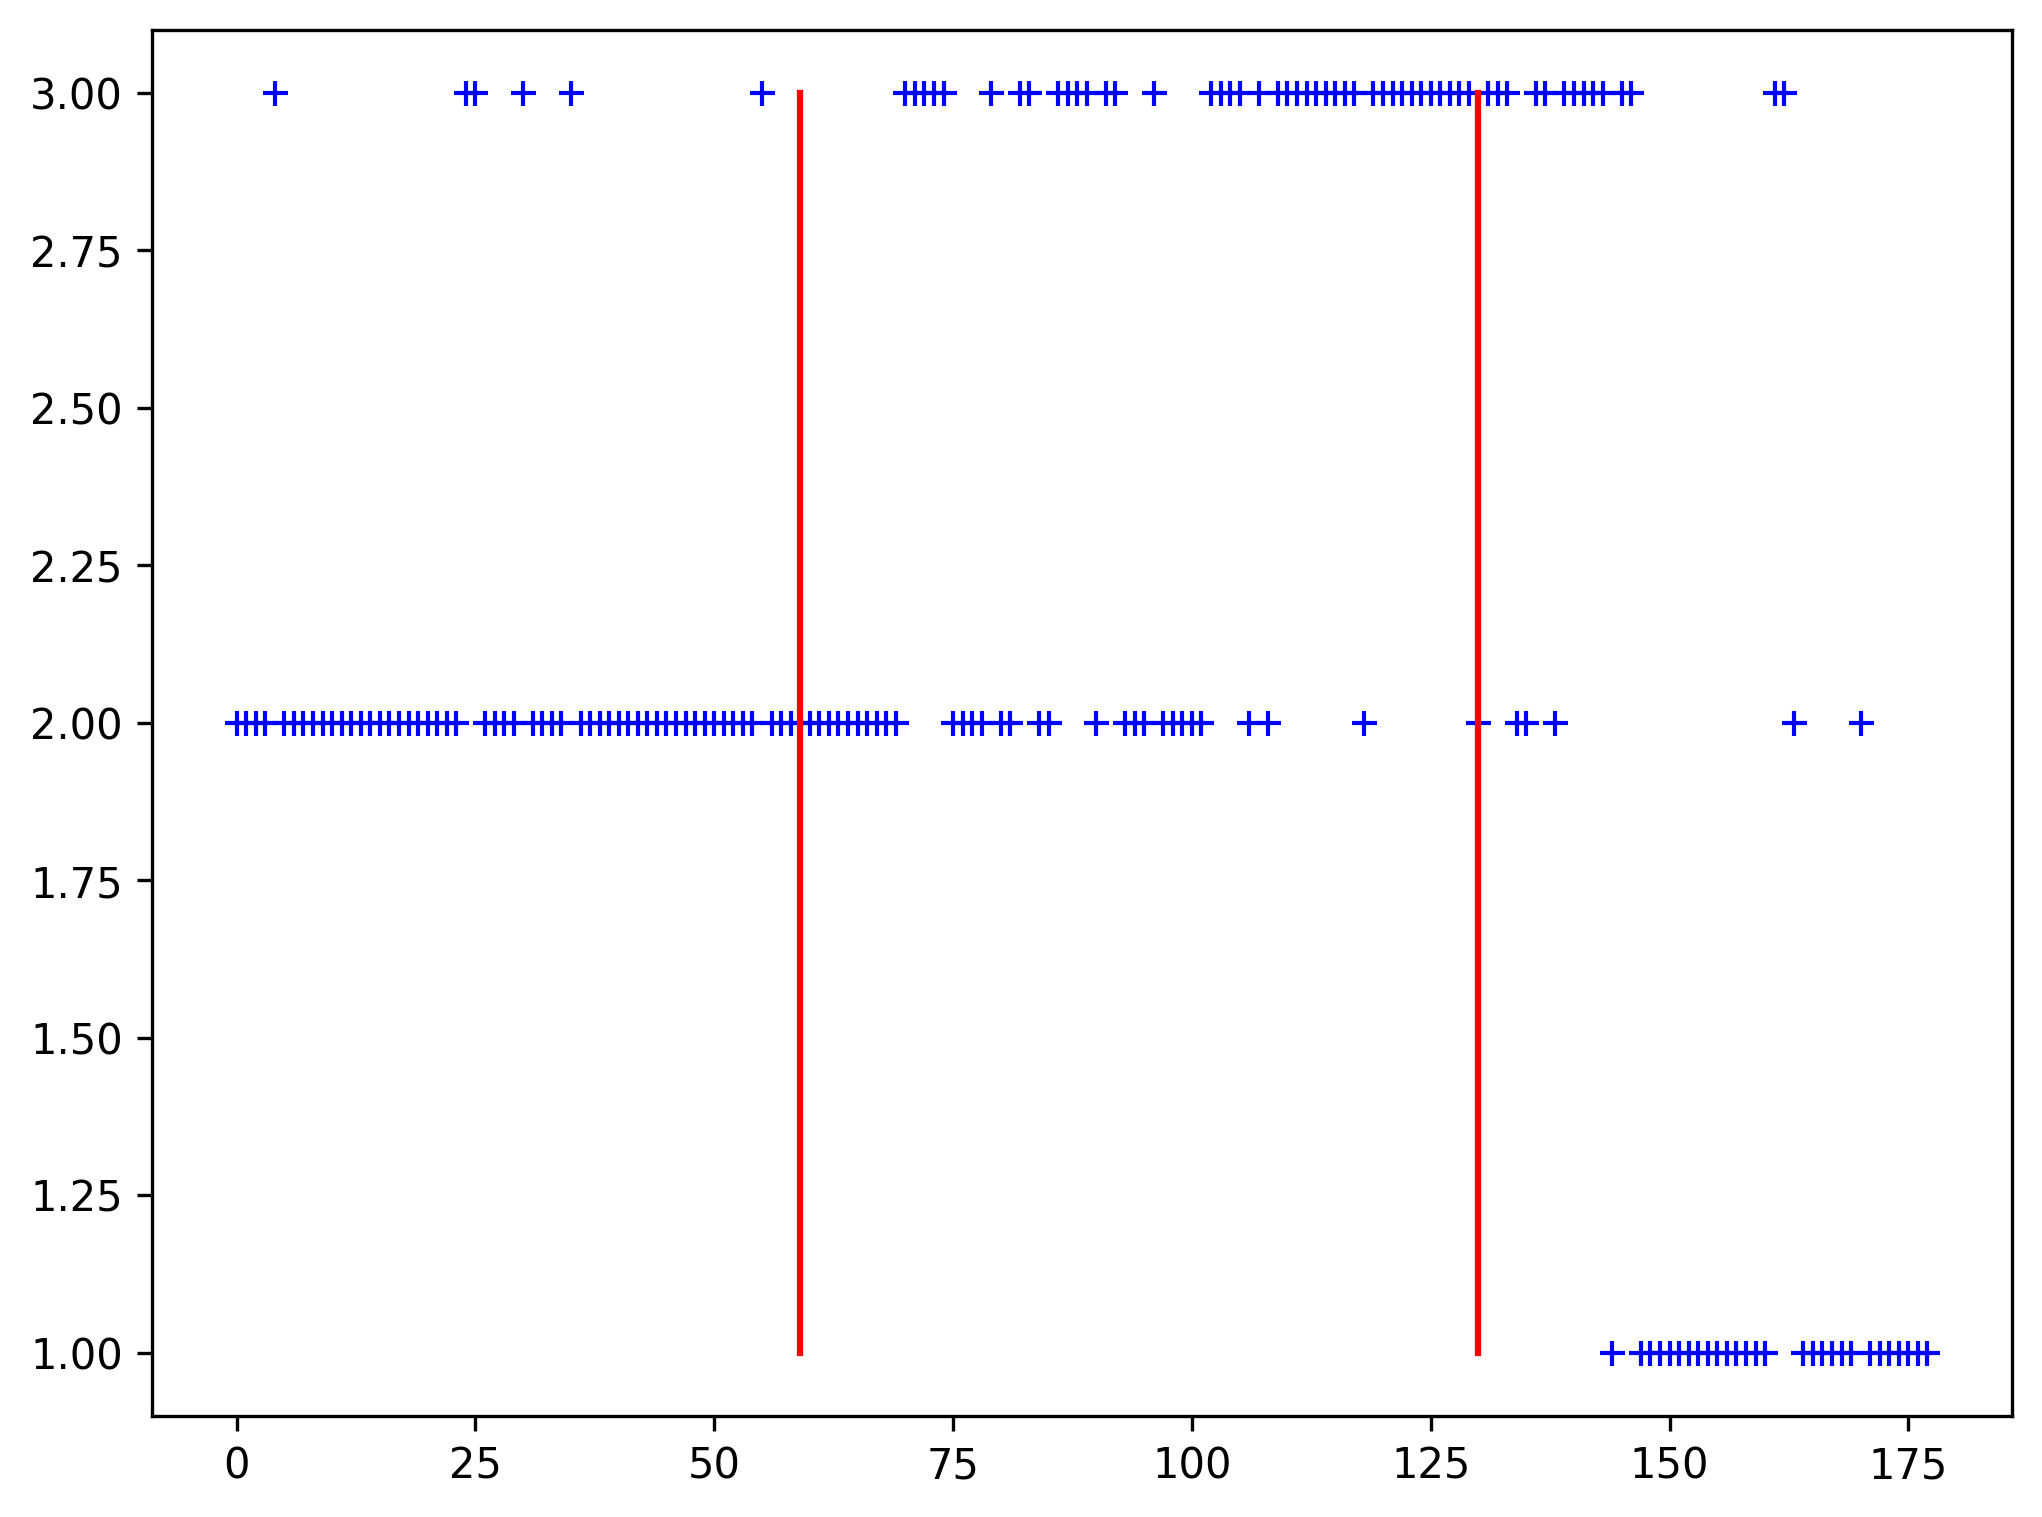
\includegraphics[width=0.6\textwidth]{normal_atributes.png} % Chemin de l'image
   \caption{Classes des données avec attributs choisis par personne lambda}
\end{figure}


Lorsqu'on regarde le taux de succès global, on a 67.84 \%.\\

On a par groupe on a :
\begin{itemize}
\item Wine-group 1 : 89.65 \%
\item Wine-group 2 : 55.55 \%
\item Wine-group 3 : 58.33 \%
\end{itemize}

\vspace{10pt}

Lorsqu'on applique KMeans avec des attributs choisis par un connaiseur on obtient :

\begin{figure}[h!] % Placement de l'image
   \centering
   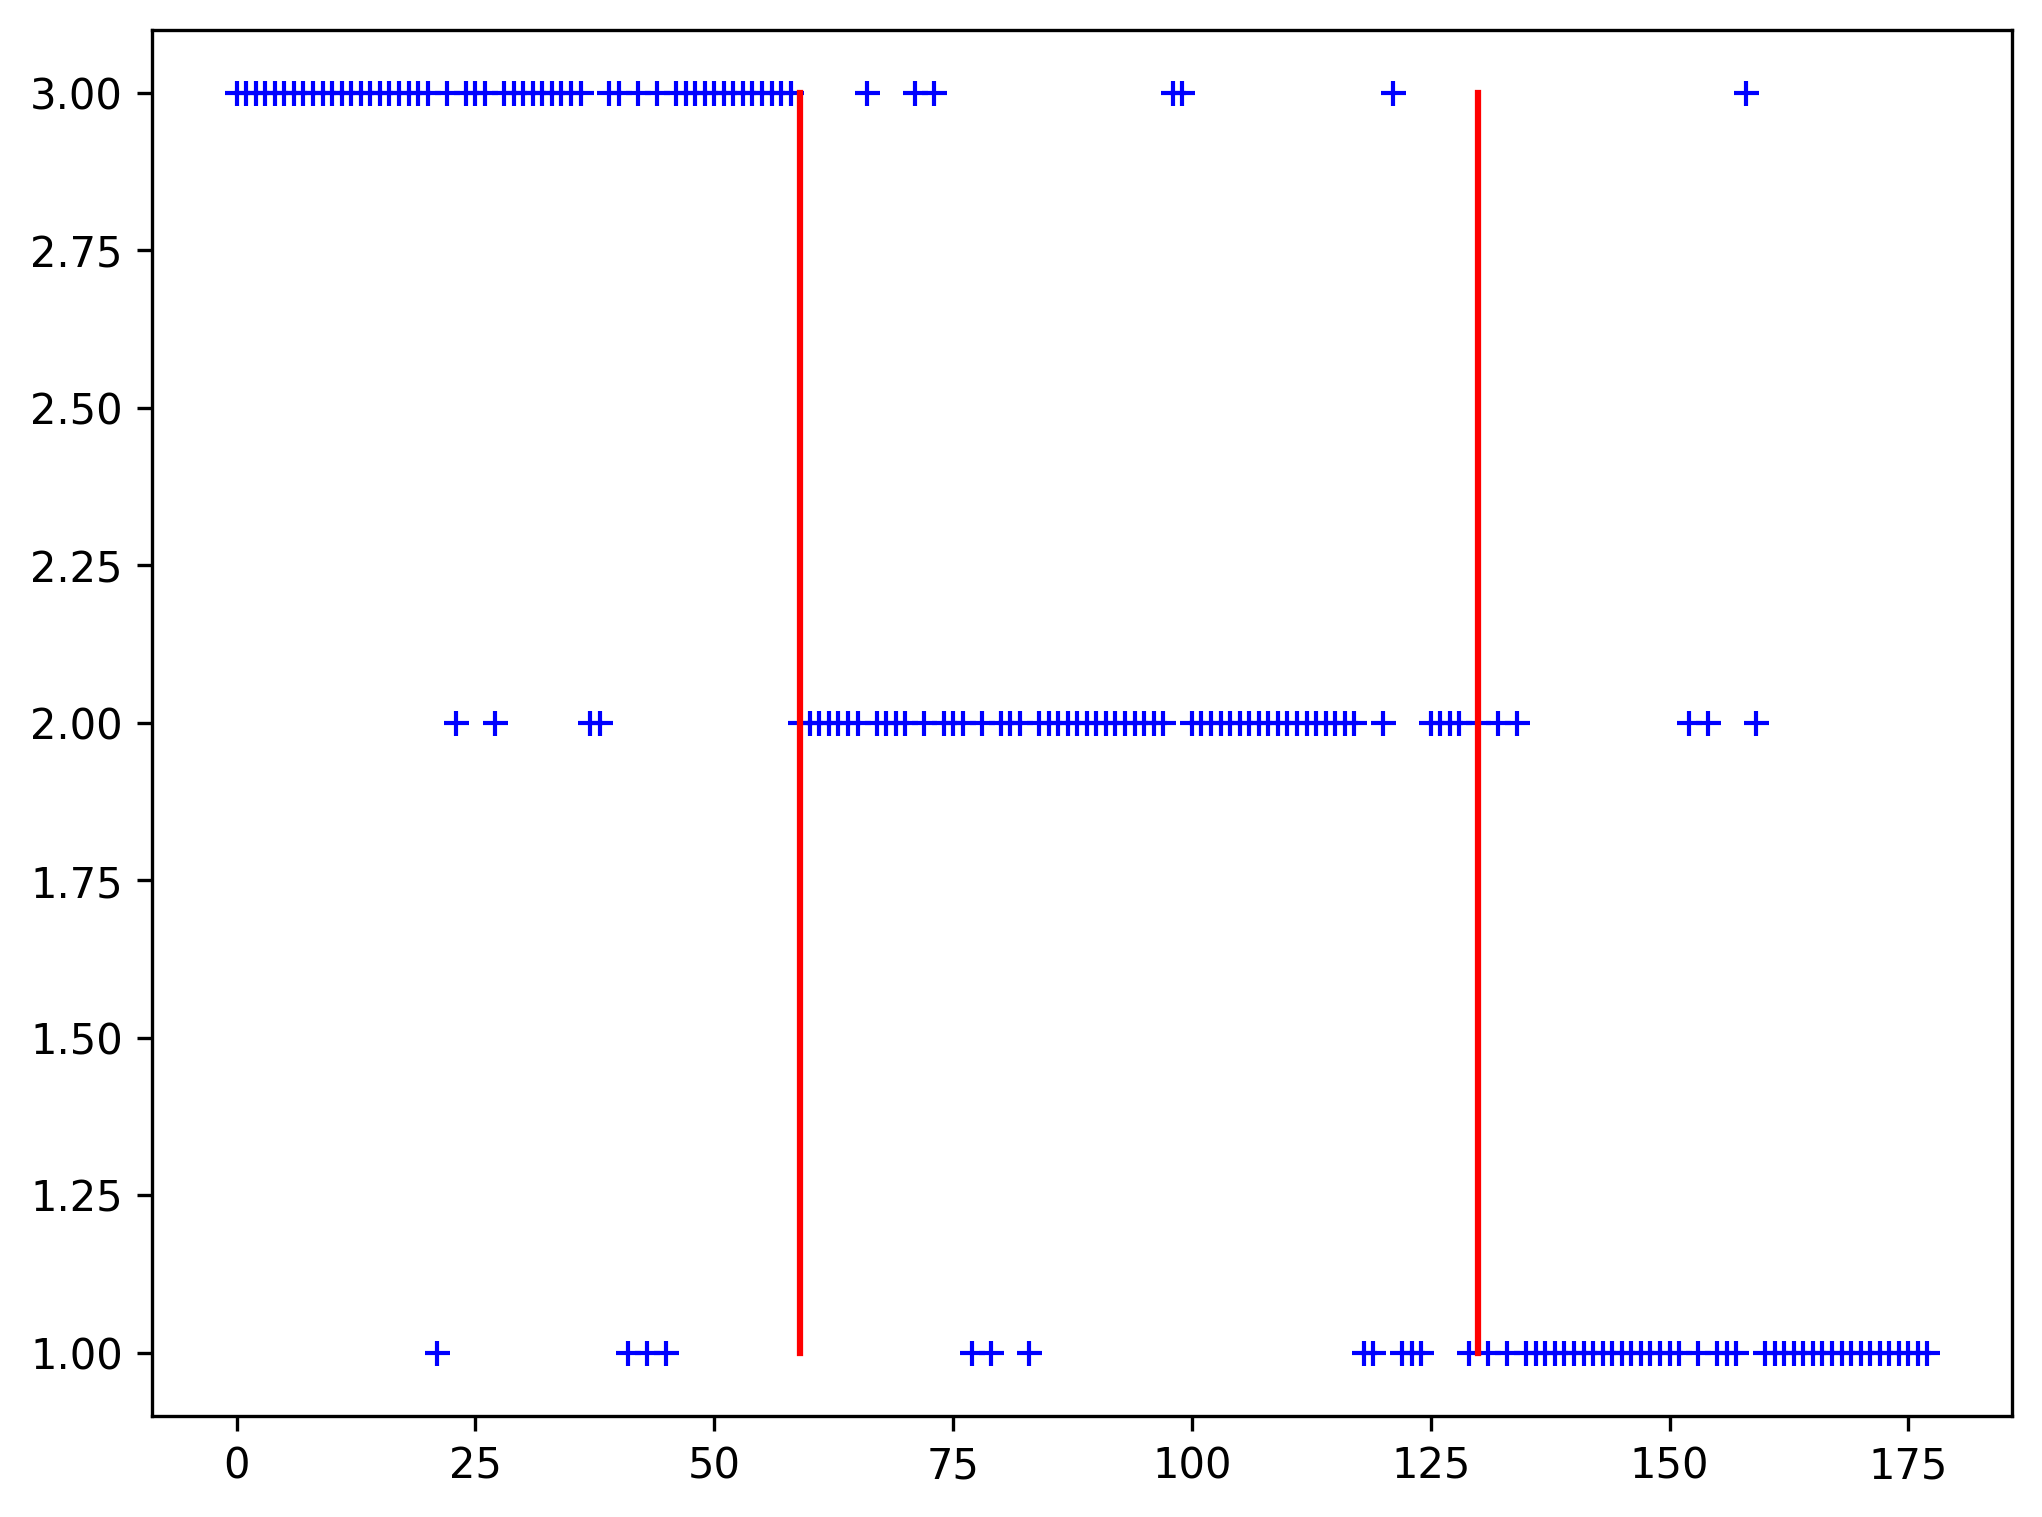
\includegraphics[width=0.6\textwidth]{profetional_atributes.png} % Chemin de l'image
   \caption{Classes des données avec attributs choisis par un connaisseur}
\end{figure}
Lorsqu'on regarde le taux de succès global, on a 83.13 \%.\\

On a par groupe on a :
\begin{itemize}
\item Wine-group 1 : 86.20 \%
\item Wine-group 2 : 77.77 \%
\item Wine-group 3 : 85.41 \%
\end{itemize}

\begin{figure}[h!] % Placement de l'image
   \centering
   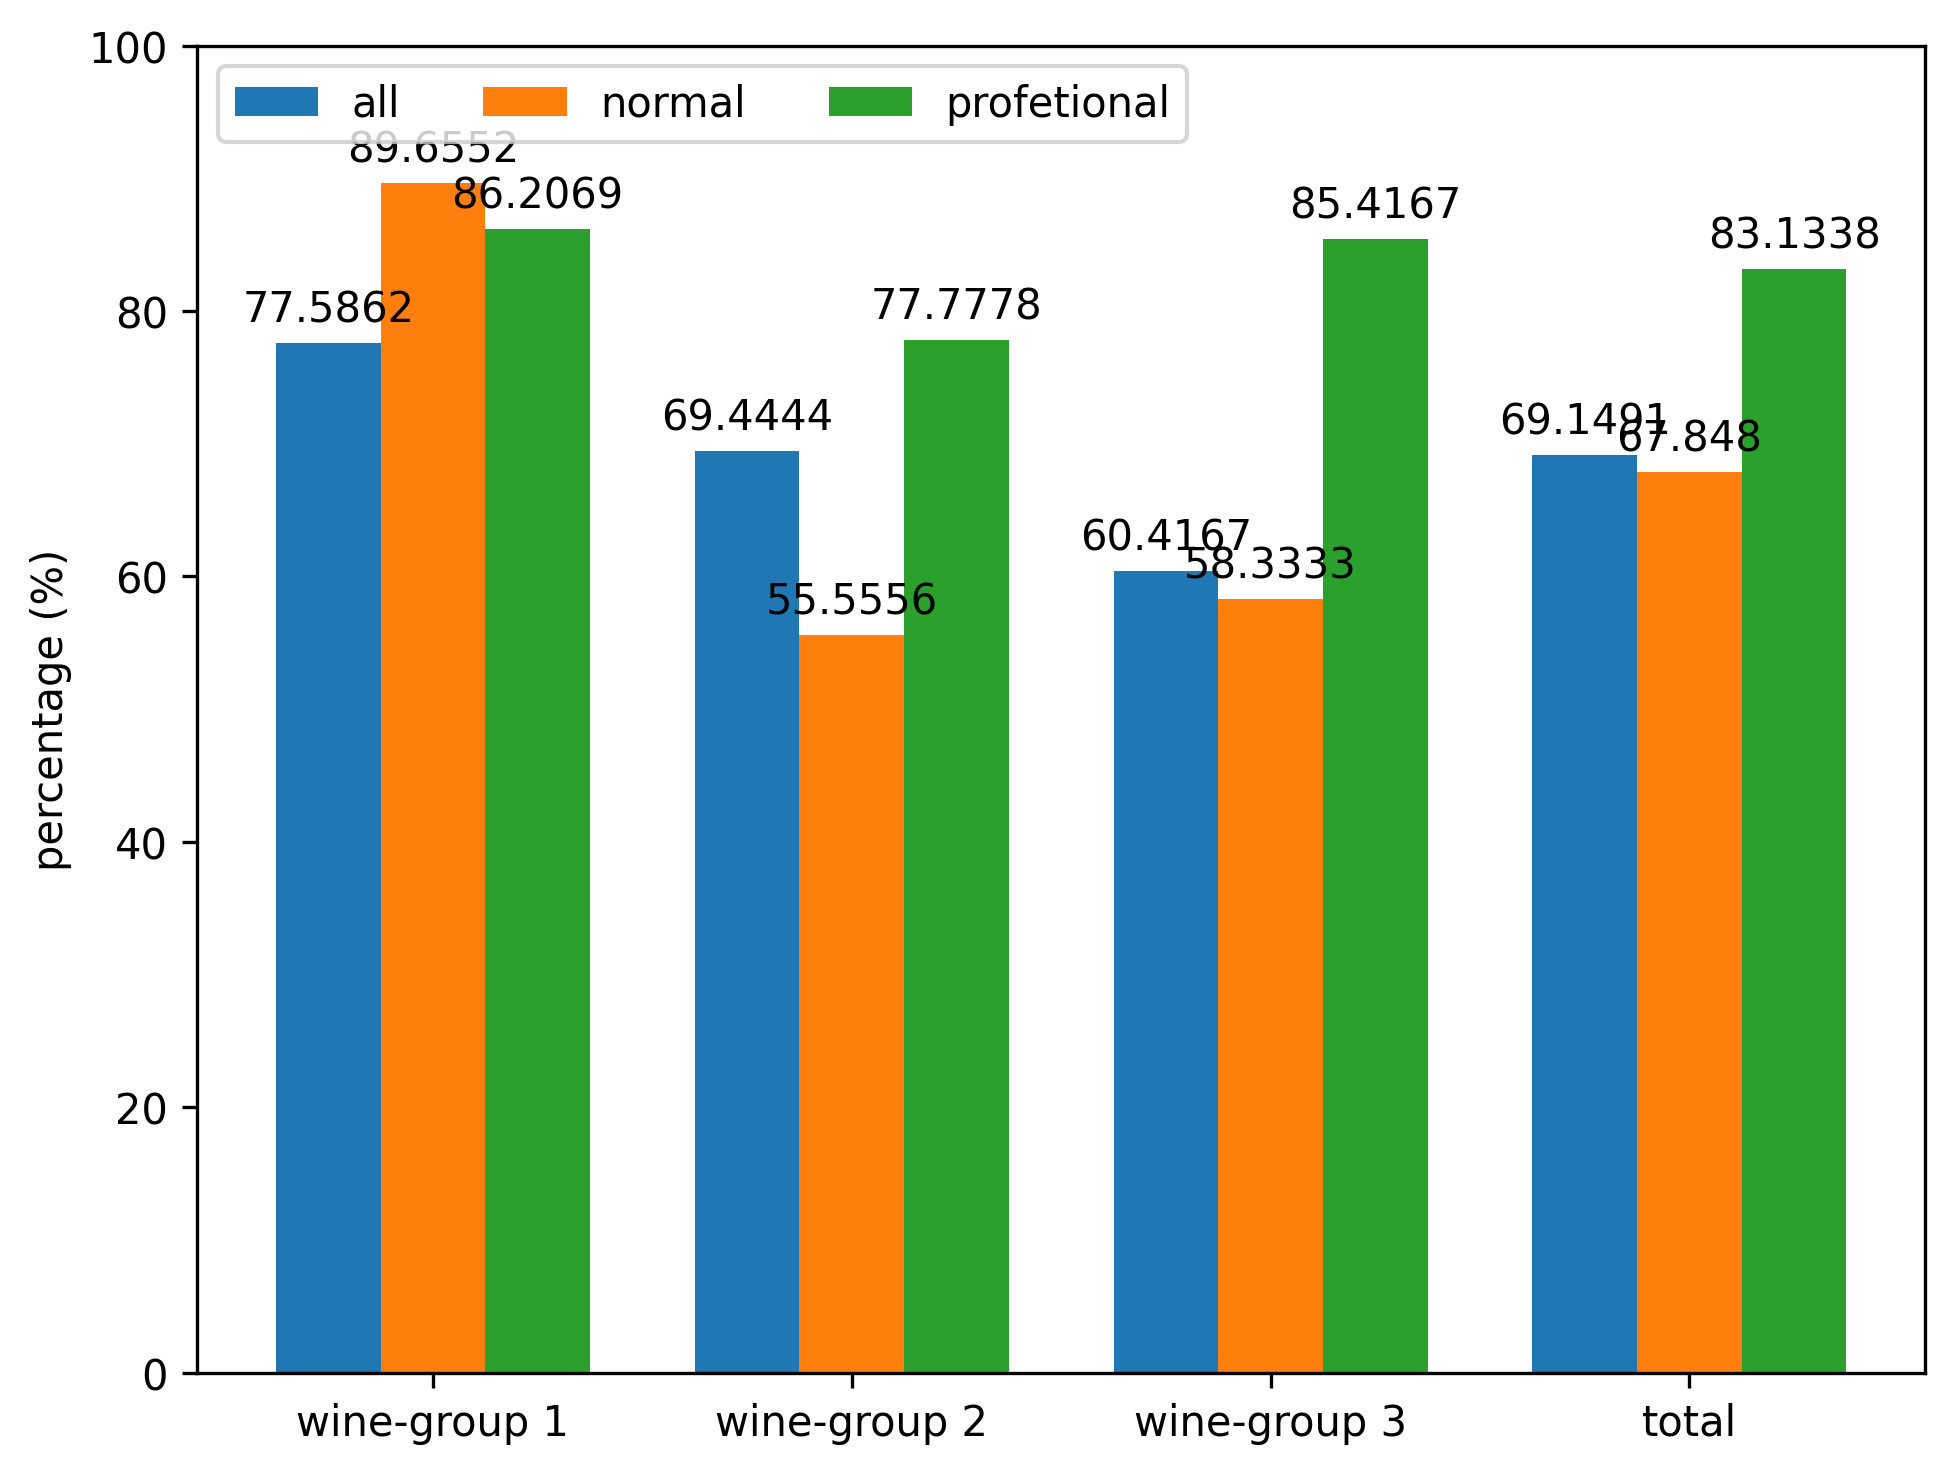
\includegraphics[width=0.6\textwidth]{differents_attributes.png} % Chemin de l'image
   \caption{Comparaison de reussite selon les attributs choisis}
   \label{fig:compare}
\end{figure}

\section{Conclusion}
\label{sec:conclusion}

Comme nous le montre la figure \ref{fig:vp}, on observe, que d'après l'ACP,  la teinte, la proline, Od280/OD315 des vins dilués, l'intensité de la couleur et les phénols non flavanoïdes n'ont pas beaucoup d'impacts par rapport aux caractéristiques.\\

On peut aussi en conclure que lorsqu'on applique l'ACP le taux de succès des deux algorithmes n'est pas très élevé : 49,44 \% pour \ref{fig:lloyd} et \ref{fig:elkan}.\\

On a essayé aussi de changer le tirage aléatoire avec des valeurs de début, et même de cette manière on obtient le même pourcentage de succès.\\

On remarque assez facilement que les attributs choisis par les professionnels sont les meilleurs \ref{fig:compare}. On comprends donc que choisir trop d'atributs n'est pas toujours la meilleure solution, mais en choisissant moins d'attributs au hasard ce n'est pas mieux.\\

Il faut donc choisir judicieusement les données que l'on veut traiter.\\

De plus on remarque que les professionnels s'y connaissent très bien du fait que leur taux de réussite est au-delà de 80\%. 
\end{document}
